\chapter{Radio definida por Software}

Cuando en telecomunicaciones se habla de radio, se hace referencia al hardware necesario para transmitir o recibir información, haciendo uso de la banda del espectro radioeléctrico ubicado en radiofrecuencia (RF).

La mayoría de los sistemas de comunicación de hoy en día necesitan de un radio: la telefonía móvil,  la navegación por satélite, la aviación comercial, la televisión abierta, son todos ejemplos. En general los radios varían en dimensiones y costos según la aplicación, pero son muy poco versátiles en cuanto a sus capacidades. Con cada actualización tecnológica que reciben las redes, por ejemplo la modernización de la red móvil de 3G a LTE, implica una renovación total del equipamiento de radio. 

El concepto de Radio Definida por Software no es nuevo, algunas de sus ideas fundacionales se publicaron en la década de los 80, impulsadas por algunos de los trabajos de Joseph Mitola \cite{mitola_SDR}. Pero ha sido el masivo desarrollo de la industria tecnológica el que ha impulsado en los últimos años la implementación de sistemas basados en SDR. 

Para implementar un equipo de radio definida por software, solo es necesario contar con una antena de radiofrecuencia, capaz de transmitir/emitir señales analógicas, y un conversor analógico-digital que alimenta de muestras a un procesador de propósito general. Es aquí donde radica la diferencia con los radios implementados en hardware, en los cuales se implementa toda una circuitería electrónica para realizar el procesamiento. La masividad de los procesadores y el auge de la programación de hoy en día, permiten implementar fácilmente un SDR, y realizar todo tipo de proyectos de distinta escala, reutilizando el equipamiento. 

Durante la realización de este proyecto, utilizamos como entorno de desarrollo para crear los bloques de procesamiento de señales al software GNU Radio\cite{GNURadio}, y como hardware utilizamos un equipo B200 del fabricante Ettus Research\cite{EttusResearch} junto con una antena telescópica genérica. 

\section{GNU Radio}

GNU Radio es un entorno de desarrollo orientado a procesamiento de señales, gratuito y de código abierto. Mediante la interconexion de bloques de procesamiento, puede usarse en conjunto con antenas de RF para desarrollar SDRs, o en una versión local en modo de simulación de sistemas.
 
La aplicación por defecto trae una amplia gama de bloques funcionales para trabajar, desde herramientas simples como filtros y ecualizadores, hasta estructuras complicadas, como lo es un transmisor DTV completo.  Existe además una gran comunidad, muy activa, que esta permanentemente publicando nuevos contenidos, para ampliar la gama de herramientas existentes en la actualidad. 

Esto se da porque al ser de código abierto, es relativamente sencillo crear bloques nuevos. El entorno soporta desarrollos de código en python y en C++, siendo este ultimo el lenguaje con el que hemos implementado nuestro transmisor gr-isdbt-tx. Si bien puede parecer un poco complejo comprender la metódologia de trabajo en GNU Radio en un principio,  una vez que comenzamos a trabajar con él y atravesamos la curva de aprendizaje, nos encontramos con una herramienta muy poderosa, y con la que es más sencillo comprender algunos de los conceptos teóricos establecidos en la norma.
Durante la carrera, nos habíamos encontrado con GNU Radio en algunas ocasiones, donde pusimos en practica algunos conceptos básicos de sistemas de comunicación. No fue hasta esta instancia, en la que pudimos encontrarnos con el potencial total de la herramienta. 

Pasaremos a desarrollar algunos de los conceptos clave para comprender el uso de GNU Radio, ejemplificando con nuestro transmisor gr-isdbt-tx

\subsection{Flowgraphs}

El flowgraph es la estructura de datos más básica del programa. Puede entenderse al mismo como si fuera una mesa de trabajo. Dentro de un flowgraph, vamos a insertar nuestras muestras desde la fuente, las vamos a procesar y las vamos a exportar, ya sea hacia un archivo o hacia el canal a través de una antena. 

\subsection{Bloques}

En GNU Radio, los datos siempre se mueven a través de bloques. Un bloque puede tener la fuente de datos, realizar operaciones sobre las muestras, puede exportar datos hacia el exterior del entorno, o puede tener toda una estructura de bloques adentro. 
Existen cuatro tipos de bloques, y de diferencian por la tasa de muestras que atraviesan el mismo. 

\textit{Bloques Sincronos (1:1)}, este bloque permite implementar funcionalidades que consuman y produzcan la misma cantidad de muestras por puerto. Los bloques sincronos pueden tener cualquier cantidad de entradas y salidas. En particular, cuando un bloque sincrono tiene 0 entradas, se tiene una fuente de datos (source). Cuando, al contrario, tiene 0 salidas, decimos que es un sumidero (sink). El bloque dispersor de energía por ejemplo, es un caso de bloque sincrono de gr-isdbt-tx. Volveremos sobre esto en el capitulo 5.

\textit{Bloques Decimadores (N:1)}, son los que producen menos muestras de las que consumen, y de forma análoga, existen también los \textit{Bloques Interpoladores (1:M)}.

Finalmente tenemos el caso general, \textit{Bloques Generales (N:M)}, en el cual no existe a priori una relación entre muestras de entrada y salida, y cada usuario debe definirlo para el bloque en particular que esta creando mediante una función llamada forecast. Uno de los mas claros casos de bloque general en nuestro transmisor, es el bloque que crea el cuadro OFDM. En tiempo de compilación, no sabemos los parámetros de transmisión que determinan la tasa de muestras. Es en tiempo de ejecución que estos valores quedan definidos, y el propio motor de GNU Radio se encarga de orquestar el flujo de datos para que todo funcione en régimen.

Para implementar el transmisor, tuvimos que separar las funcionalidades en bloques de procesamiento, e implementar aquellos bloques que no estuviesen ya presentes en el software. Algunos ejemplos como conversores serie a paralelo, el codificador Reed Solomon, el codificador Viterbi, existían ya como bloques funcionales del programa, y fueron re utilizados. 

\section{El flujo de datos en GNU Radio}

Para el desarrollo de los bloques de gr-isdbt-tx fue necesario comprender el modo en el que los datos se mueven entre bloques en GNU Radio. El motor del programa realiza llamados de forma periódica a los bloques en el flowgraph, dependiendo de la cantidad de muestras que tenga en cola para procesar en cada bloque, y de la tasa de muestras que busque mantener constante a través del sistema, le comunica a cada bloque la cantidad de datos que necesita que le dejen en salida.  

Al momento de crear un nuevo bloque, debemos especificar en la firma de la función, los parámetros necesarios para que el motor central pueda controlar el flujo de datos de nuestro nuevo bloque. Para realizar esto, se utilizan ciertos parámetros, precargados en la estructura de funciones de la clase, orientados a la entrada/salida de datos, estos son,  noutputitems y ninputitems. 

Mediante estas variables, el motor de procesamiento puede obligar a los bloques a ejecutarse mas de una vez en cada llamado, pues exige la cantidad de salidas que necesita para mantener la tasa. Para esto, le notifica al bloque en la variable noutputitems, la cantidad de “tandas” de datos que la instancia actual del bloque necesita devolverle al motor de procesamiento para mantener la tasa. 

La variable ninputitems, mantiene el control de la cantidad de datos que hay en cada uno de los puertos de entrada. Y utilizándola como variable, podemos especificar cuantos datos de entrada precisamos consumir para obtener un dato en el puerto de salida.

Esta operación depende bastante de la naturaleza del bloque, por ejemplo, en los bloques síncronos, se sabe de antemano que la tasa de muestras se mantendrá constante, por lo que alcanza con especificar el tipo y la cantidad de muestras que atravesarán el bloque en una ejecución. 

Los bloques de tipo general, son mas complicados, pues es necesario especificar explícitamente la relación entre la cantidad de muestras a la entrada y a la salida. Este control de flujo se realiza desde un método, precargado en la clase con la que se crea el bloque, denominado forecast.

\section{Hardware}
Universal Software Radio Peripheral (USRP) es una linea de plataformas de hardware para SDRs diseñados y comercializados por la empresa Ettus Research. Gran parte de la arquitectura de estos equipos es de código abierto, y puede ser descargada desde la web de la empresa. Con estos equipos se logra poner en funcionamiento soluciones de radio definida por software por costo accesible, ya que la gama de precios de los equipos de la compañia oscila en un entorno de 1000 dólares. 

Tambien existen otros proveedores de menor renombre, con equipos que presentan un desempeño un poco mas ruidoso, como es el caso del HackRF que comercializa Great Scott Gadgets\cite{GreatScottGadgets}, en el entorno de los 300 dólares. Durante el desarrollo de gr-isdbt-tx experimentamos con el modelo HackRF One, con magros resultados, por lo que no consideramos pertinente detallar mas sobre el mismo. Aunque para otras aplicaciones de SDR, se ha probado que funciona de manera correcta.

En lineas generales, se componen de una placa madre en la que conviven varios subsistemas, como lo son un generador y sincronizador de señales de reloj, conversores analógico digitales y FPGAs, que se encargan de realizar tareas de procesamiento de señal en banda base. Se complementa con una placa modular denominada “daughterboard” que realiza tareas como filtrado, condicionamiento de señal y modulación las señales en frecuencias de hasta 6 GHz.

\begin{figure}[h!]
	\centering
	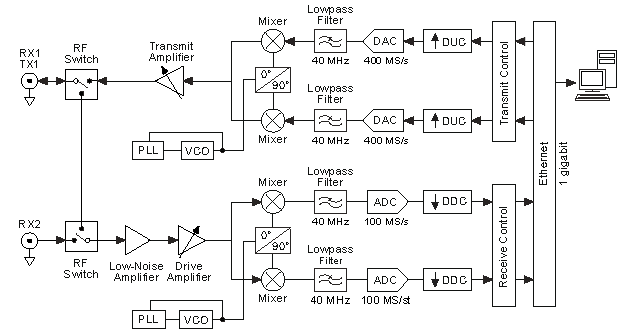
\includegraphics[scale=0.55]{figuras/cap04/usrp_arq}
	\caption{\label{f:usrp_arq} Arquitectura general de un equipo USRP\cite{USRP_arch}}
\end{figure}

Durante este proyecto, trabajamos con el modelo USRP B100 de Ettus Research. A continuación presentamos una breve reseña del equipo.

\subsection{USRP B100}

En este modelo, las muestras llegan al equipo a través de una interfaz USB 2.0 y tiene una capacidad para transmitir en velocidades de hasta 128 MS/s (Mega Samples per Second), cuando se trabaja con muestras de 14 bits. Esta limitacion del equipo viene del conversor DAC con el que convertiremos las muestras para transmitir, para trabajar en recepcion, el limite se da por el conversor ADC que soporta hasta 64 MS/s con muestras de hasta 12 bits. Por ultimo, el ancho de banda con el que se puede trabajar con el B100 es de hasta 8MHz, trabajando con muestras de 16 bits.\cite{b100}  

Este modelo en particular esta actualmente discontinuado, pero su precio en el mercado rondaba los 700 dolares. Para el desarrollo del proyecto, recibimos en calidad de préstamo uno de estos equipos para las pruebas

Para poder levantar el equipo desde una PC, es necesario instalar el driver universal de Ettus, “USRP Hardware Driver”. La mejor forma de hacer esto es instalarlo desde su repositorio oficial \cite{UHD}. El driver es gratuito y de codigo abierto, y soporta todos los equipos de radio de Ettus.


\subsubsection{Interfaz con GNU Radio}

Para intercomunicar al equipo con el software de procesamiento de datos, es necesario incluir en el flowgraph los bloques del complemento gr-uhd (en las versiones actuales de GNU Radio ya vienen incluidos). El bloque sink de este complemento vincula al flujo de datos del software con el puerto receptor de datos del equipo, y permite especificar los parámetros de transmision como frecuencia central y ancho de banda.

\begin{figure}[h!]
	\centering
	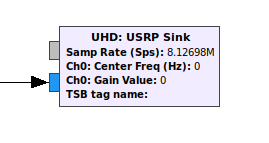
\includegraphics[scale=0.55]{figuras/cap04/sink_block}
	\caption{\label{f:sink_block} Bloque sink al equipo USRP}
\end{figure}

Los argumentos con los que funciona son la tasa de muestras, la frecuencia de destino en la que se desea transmitir y el valor de ganancia aplicado a la señal de entrada. Es importante verificar que los parametros a seleccionar sean soportados por el hardware. En el caso de nuestro transmision, tiene una tasa de muestras objetivo de:

\begin{gather*}
	f_{IFFT} = \frac{portadoras}{T_{s}} = \frac{512}{63} \approx 8.127 MHz
\end{gather*}

Para verificar que la tasa de muestras sea soportada por el transmisor, primero debemos verificar el tamaño de los datos. En nuestro caso, el tipo es \textit{grc::complex}, el cual es un tipo propio de GNU Radio, formado por una unión de dos variables \textit{std::complex} cada una de 32 bits representadas en punto flotante. Es decir que cada una de las muestras de nuestro transmisor se compone de 64 bits.

Un aspecto a tener en cuenta con el transmisor, es verificar que la amplitud de las muestras esté normalizada, a modo de evitar un efecto de \textit{clipping} a la salida, esto es, que todas las muestras superiores a 1, terminaran con la misma amplitud en recepción, lo que nos dejará una señal trunca en amplitud. Evitar este problema resulta sencillo, basta con agregar una ganancia a la salida del sistema controlado por una variable, y verificar para que valores de la misma que la señal en el tiempo este en el rango esperado.